\documentclass[border=2pt]{standalone}
\usepackage{amsmath,amssymb}
% Shared visual language for the figures of the book.
% Every figure in this directory loads this file so the chapter reads as one system.
% NOTE: no blank lines are allowed inside \tikzset{...} (a blank line emits \par
% and breaks key scanning).
\NeedsTeXFormat{LaTeX2e}
\ProvidesPackage{figstyle}[2026/10/21 Figure style for Free Energy to LLMs]

\RequirePackage{tikz}
\usetikzlibrary{arrows.meta,positioning,calc,fit,shapes.geometric,shapes.misc,%
  backgrounds,matrix,decorations.pathreplacing,decorations.markings,patterns.meta}

% ---------------------------------------------------------------- palette
% Same values as book/preamble/style.tex, prefixed with F.
\definecolor{FNavy}{HTML}{14324A}
\definecolor{FTeal}{HTML}{0E7490}
\definecolor{FSky}{HTML}{E7F5F8}
\definecolor{FOrange}{HTML}{D97706}
\definecolor{FAmber}{HTML}{FFF3D6}
\definecolor{FInk}{HTML}{1F2937}
\definecolor{FSlate}{HTML}{64748B}
\definecolor{FMist}{HTML}{F5F7FA}
\definecolor{FRose}{HTML}{9F1239}
\definecolor{FRoseMist}{HTML}{FFF1F2}

% ---------------------------------------------------------------- semantics
% Teal   = probability / model / data object
% Orange = training objective, cost, or the quantity moved through the system
% Navy   = neutral structure
% Slate  = secondary label or metadata
% Rose   = failure mode, hazard, masked-out region
\tikzset{
  % Lay figures out in millimetres.  A figure designed 168mm wide is included at
  % \textwidth, so its fonts appear at exactly the size written here.
  every picture/.style={x=1mm,y=1mm,font=\small,line cap=round,line join=round},
  % ---- block styles
  nbase/.style={draw,rounded corners=1.2pt,align=center,inner sep=2.4pt,%
    minimum height=7mm,text=FInk},
  nteal/.style={nbase,draw=FTeal,fill=FSky},
  norange/.style={nbase,draw=FOrange,fill=FAmber},
  nnavy/.style={nbase,draw=FNavy,fill=white},
  nsoft/.style={nbase,draw=FSlate!55,fill=FMist},
  nrose/.style={nbase,draw=FRose,fill=FRoseMist},
  ghost/.style={draw=none,fill=none,align=center,inner sep=1pt},
  plain/.style={draw=none,fill=none,align=center,inner sep=0pt},
  % ---- arrows
  ar/.style={-{Latex[length=1.7mm,width=1.35mm]},draw=FSlate,line width=0.75pt},
  ard/.style={ar,dashed},
  arteal/.style={ar,draw=FTeal},
  arorange/.style={ar,draw=FOrange},
  arrose/.style={ar,draw=FRose},
  thickar/.style={ar,line width=1.2pt},
  % ---- text roles
  ftitle/.style={font=\large\bfseries,text=FNavy,align=center},
  ptitle/.style={font=\small\bfseries,text=FNavy,align=center},
  ptitleo/.style={font=\small\bfseries,text=FOrange,align=center},
  lbl/.style={font=\scriptsize,text=FSlate,align=center,inner sep=1pt},
  lblt/.style={lbl,text=FTeal},
  lblo/.style={lbl,text=FOrange},
  lbln/.style={lbl,text=FNavy},
  lblr/.style={lbl,text=FRose},
  sub/.style={font=\scriptsize,text=FSlate!90,align=center,inner sep=1pt},
  monob/.style={font=\ttfamily\scriptsize,text=FInk,inner sep=1pt},
  mathb/.style={font=\small,text=FInk,inner sep=1pt},
  eqn/.style={font=\scriptsize,inner sep=1.5pt,text=FInk},
  % ---- decorations
  brace/.style={decorate,decoration={brace,amplitude=2.4pt},draw=FSlate,%
    line width=0.6pt},
  bracet/.style={brace,draw=FTeal},
  braceo/.style={brace,draw=FOrange},
  axis/.style={draw=FSlate!55,line width=0.6pt},
  guide/.style={draw=FSlate!45,line width=0.5pt,dashed},
  halolabel/.style={font=\scriptsize,text=FInk,fill=white,fill opacity=0.85,%
    text opacity=1,inner sep=1.4pt,align=center},
}

% Figure title above the drawing, anchored at the figure's top-left.
\newcommand{\figtitle}[2][0]{%
  \node[ftitle,anchor=north west,outer sep=0pt] at (#1,0) {#2};}

% Rounded panel behind a subgroup of nodes.
\newcommand{\figpanel}[3][]{%
  \node[draw=FSlate!35,fill=#3,rounded corners=2pt,inner sep=2.6mm,#1] {#2};}

\endinput

\begin{document}
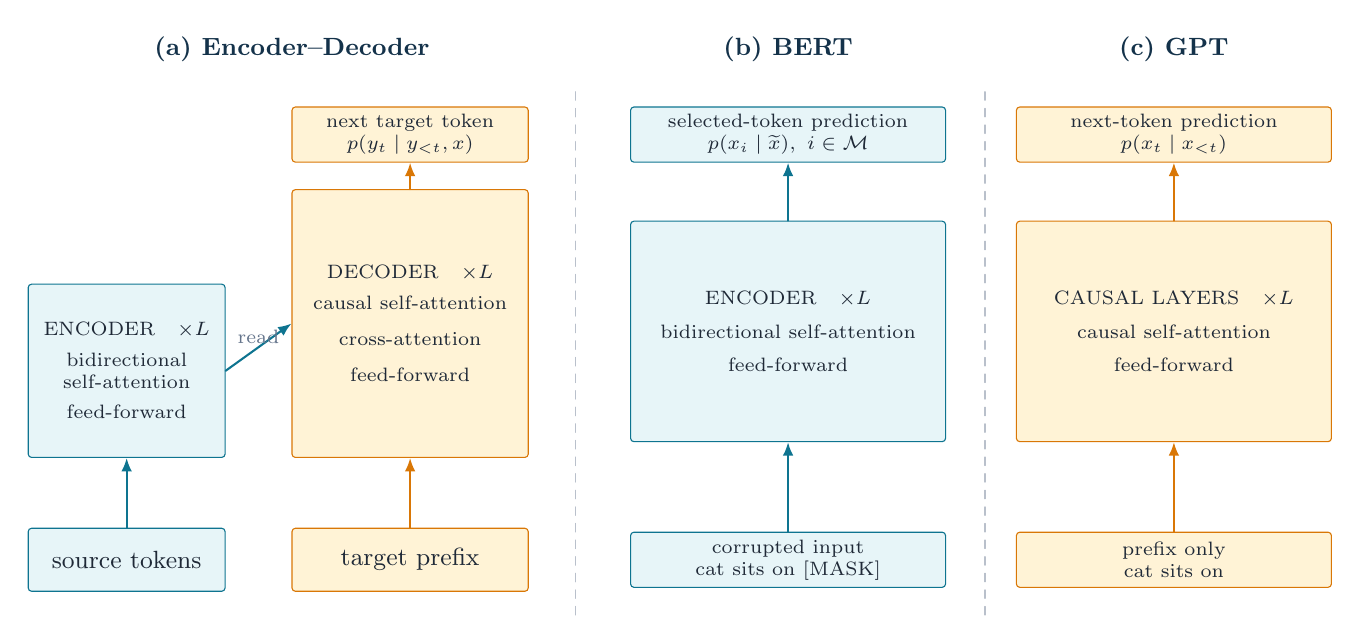
\begin{tikzpicture}
% Full-page teaching diagram, three distinct routes; read bottom to top.
\node[ptitle,anchor=south] at (34,69) {(a) Encoder--Decoder};
\node[ptitle,anchor=south] at (97,69) {(b) BERT};
\node[ptitle,anchor=south] at (146,69) {(c) GPT};
\draw[guide] (70,0)--(70,67);\draw[guide] (122,0)--(122,67);
\node[nteal,minimum width=25mm,minimum height=8mm] (src) at (13,7) {source tokens};
\node[norange,minimum width=30mm,minimum height=8mm] (tgt) at (49,7) {target prefix};
\node[nteal,minimum width=25mm,minimum height=22mm,font=\scriptsize] (enc) at (13,31) {ENCODER\quad$\times L$\\[3pt]bidirectional\\self-attention\\[3pt]feed-forward};
\node[norange,minimum width=30mm,minimum height=34mm,font=\scriptsize] (dec) at (49,37) {DECODER\quad$\times L$\\[3pt]causal self-attention\\[5pt]cross-attention\\[5pt]feed-forward};
\draw[arteal] (src)--(enc);
\draw[arorange] (tgt)--(dec);
\draw[arteal] (enc.east)--node[lbl,above,rotate=0]{read}(dec.west);
\node[norange,minimum width=30mm,font=\scriptsize] (out) at (49,61) {next target token\\$p(y_t\mid y_{<t},x)$};
\draw[arorange] (dec)--(out);
\node[nteal,minimum width=40mm,font=\scriptsize] (bi) at (97,7) {corrupted input\\cat sits on [MASK]};
\node[nteal,minimum width=40mm,minimum height=28mm,font=\scriptsize] (be) at (97,36) {ENCODER\quad$\times L$\\[4pt]bidirectional self-attention\\[4pt]feed-forward};
\node[nteal,minimum width=40mm,font=\scriptsize] (bo) at (97,61) {selected-token prediction\\$p(x_i\mid\widetilde x),\ i\in\mathcal M$};
\draw[arteal] (bi)--(be);\draw[arteal] (be)--(bo);
\node[norange,minimum width=40mm,font=\scriptsize] (gi) at (146,7) {prefix only\\cat sits on};
\node[norange,minimum width=40mm,minimum height=28mm,font=\scriptsize] (ge) at (146,36) {CAUSAL LAYERS\quad$\times L$\\[4pt]causal self-attention\\[4pt]feed-forward};
\node[norange,minimum width=40mm,font=\scriptsize] (go) at (146,61) {next-token prediction\\$p(x_t\mid x_{<t})$};
\draw[arorange] (gi)--(ge);\draw[arorange] (ge)--(go);
\end{tikzpicture}
\end{document}
